% Options for packages loaded elsewhere
\PassOptionsToPackage{unicode}{hyperref}
\PassOptionsToPackage{hyphens}{url}
\documentclass[
  11pt,
  a4paper,
]{article}
\usepackage{xcolor}
\usepackage[margin=22mm]{geometry}
\usepackage{amsmath,amssymb}
\setcounter{secnumdepth}{-\maxdimen} % remove section numbering
\usepackage{iftex}
\ifPDFTeX
  \usepackage[T1]{fontenc}
  \usepackage[utf8]{inputenc}
  \usepackage{textcomp} % provide euro and other symbols
\else % if luatex or xetex
  \usepackage{unicode-math} % this also loads fontspec
  \defaultfontfeatures{Scale=MatchLowercase}
  \defaultfontfeatures[\rmfamily]{Ligatures=TeX,Scale=1}
\fi
\usepackage{lmodern}
\ifPDFTeX\else
  % xetex/luatex font selection
\fi
% Use upquote if available, for straight quotes in verbatim environments
\IfFileExists{upquote.sty}{\usepackage{upquote}}{}
\IfFileExists{microtype.sty}{% use microtype if available
  \usepackage[]{microtype}
  \UseMicrotypeSet[protrusion]{basicmath} % disable protrusion for tt fonts
}{}
\makeatletter
\@ifundefined{KOMAClassName}{% if non-KOMA class
  \IfFileExists{parskip.sty}{%
    \usepackage{parskip}
  }{% else
    \setlength{\parindent}{0pt}
    \setlength{\parskip}{6pt plus 2pt minus 1pt}}
}{% if KOMA class
  \KOMAoptions{parskip=half}}
\makeatother
\usepackage{longtable,booktabs,array}
\newcounter{none} % for unnumbered tables
\usepackage{calc} % for calculating minipage widths
% Correct order of tables after \paragraph or \subparagraph
\usepackage{etoolbox}
\makeatletter
\patchcmd\longtable{\par}{\if@noskipsec\mbox{}\fi\par}{}{}
\makeatother
% Allow footnotes in longtable head/foot
\IfFileExists{footnotehyper.sty}{\usepackage{footnotehyper}}{\usepackage{footnote}}
\makesavenoteenv{longtable}
\usepackage{graphicx}
\makeatletter
\newsavebox\pandoc@box
\newcommand*\pandocbounded[1]{% scales image to fit in text height/width
  \sbox\pandoc@box{#1}%
  \Gscale@div\@tempa{\textheight}{\dimexpr\ht\pandoc@box+\dp\pandoc@box\relax}%
  \Gscale@div\@tempb{\linewidth}{\wd\pandoc@box}%
  \ifdim\@tempb\p@<\@tempa\p@\let\@tempa\@tempb\fi% select the smaller of both
  \ifdim\@tempa\p@<\p@\scalebox{\@tempa}{\usebox\pandoc@box}%
  \else\usebox{\pandoc@box}%
  \fi%
}
% Set default figure placement to htbp
\def\fps@figure{htbp}
\makeatother
\setlength{\emergencystretch}{3em} % prevent overfull lines
\providecommand{\tightlist}{%
  \setlength{\itemsep}{0pt}\setlength{\parskip}{0pt}}
\usepackage{bookmark}
\IfFileExists{xurl.sty}{\usepackage{xurl}}{} % add URL line breaks if available
\urlstyle{same}
\hypersetup{
  pdftitle={From many logarithms to two{,} and the unit equation},
  pdfauthor={GPT-6 Astra (OpenAI), Ultra},
  hidelinks,
  pdfcreator={LaTeX via pandoc}}

\title{From many logarithms to two, and the unit equation}
\author{GPT-6 Astra (OpenAI), Ultra}
\date{October 2026}

\providecommand{\Eta}{\mathrm{H}}
\begin{document}
\maketitle

\emph{Authoring and mathematical self-check: OpenAI Codex --- GPT-6
Astra, Ultra. Original exposition, CC0.}

The coefficient normalization in Theorem 7.1 has an application beyond
two fixed bases. We can replace a long logarithmic sum by a two-term sum
whose bases vary in a controlled way. One base becomes more complicated
as the common multiplier decreases; the other becomes less complicated.
The product of their height bounds is what matters.

The free paper of
\href{https://numdam.org/item/JTNB_2000__12_1_13_0/}{Bilu and Bugeaud,
Section 2} gives the geometric reduction underlying this argument. We
give all the rounding estimates and an explicit, deliberately generous
constant. The arithmetic inputs are the height inequalities in
\emph{Heights of algebraic numbers}, Proposition 2.5 and Theorem 2.8,
already used in Lesson 1. The analytic input is our proved Theorem 7.1,
including its allowance for arbitrary complex logarithms and
multiplicative dependence.

\subsection{Prerequisite proofs}\label{prerequisite-proofs}

The following programme lessons provide the inputs used here.

{\def\LTcaptype{none} % do not increment counter
\begin{longtable}[]{@{}
  >{\raggedright\arraybackslash}p{(\linewidth - 2\tabcolsep) * \real{0.5000}}
  >{\raggedright\arraybackslash}p{(\linewidth - 2\tabcolsep) * \real{0.5000}}@{}}
\toprule\noalign{}
\begin{minipage}[b]{\linewidth}\raggedright
Input
\end{minipage} & \begin{minipage}[b]{\linewidth}\raggedright
Exact proof locator
\end{minipage} \\
\midrule\noalign{}
\endhead
\bottomrule\noalign{}
\endlastfoot
Mahler measure, height inequalities, Northcott, height zero and
one-place estimates & \href{https://kokunoyumeto.github.io/open-math-courses-public/courses/TR-TRANS/TR-TRANS-02.html}{Heights of
algebraic numbers, Theorems 2.4 and 2.6--2.8, Proposition 2.5} \\
Integer subgroup bases, saturation and integral bases &
\href{https://kokunoyumeto.github.io/open-math-courses-public/courses/NT-ANT/discriminants-and-integral-bases.html\#integer-subgroups-and-lattice-indices}{Discriminants
and integral bases, Integer subgroups and lattice indices; Theorem
2.3} \\
Ideal norms and the norm of a principal ideal &
\href{https://kokunoyumeto.github.io/open-math-courses-public/courses/NT-ANT/norms-class-groups-and-modules-over-dedekind-domains.html}{Norms,
class groups and modules over Dedekind domains, Proposition 4.1} \\
Discrete subgroups and the compact Minkowski theorem &
\href{https://kokunoyumeto.github.io/open-math-courses-public/courses/NT-ANT/lattices-minkowskis-theorem-and-the-minkowski-embedding.html}{Lattices,
Minkowski's theorem and the Minkowski embedding, lattice structure lemma
and Theorem 7.1} \\
Dirichlet's theorem, the regulator and the \(S\)-unit rank &
\href{https://kokunoyumeto.github.io/open-math-courses-public/courses/NT-ANT/dirichlets-unit-theorem.html}{Dirichlet's unit
theorem, Results 9.2--9.4} \\
Complex logarithm branches and the two-logarithm estimate &
\href{https://kokunoyumeto.github.io/open-math-courses-public/courses/TR-BAKER/TR-BAKER-01.html}{Lesson 1, Lemmas 1.1--1.2};
\href{https://kokunoyumeto.github.io/open-math-courses-public/courses/TR-BAKER/TR-BAKER-07.html\#1-an-explicit-bound-without-multiplicative-independence}{Lesson
7, Theorem 7.1} \\
\end{longtable}
}

\subsection{1. A common multiplier with small integral
remainders}\label{a-common-multiplier-with-small-integral-remainders}

\textbf{Lemma 12.1.} Let \(b_1,\ldots,b_n\) be integers, where
\(n\ge1\), and let \(N\ge Q\ge1\) be integers. There are integers
\(r,p_1,\ldots,p_n\) such that \[
1\le\left\lfloor\frac NQ\right\rfloor\le r\le N,
\qquad
|b_i-rp_i|\le rQ^{-1/n}+\frac{|b_i|}{2r-1}
\quad(1\le i\le n).
\tag{12.1}
\]

\textbf{Proof.} First suppose \(Q>1\). In \(\mathbb R^{n+1}\), consider
the closed region \[
|t|\le Q,\qquad
\left|\frac{tb_i}{N}-x_i\right|\le Q^{-1/n}
\quad(1\le i\le n).
\tag{12.2}
\] It is compact, convex and symmetric about zero. The shear
\((t,x_1,\ldots,x_n)\mapsto(t,x_1-tb_1/N,\ldots,x_n-tb_n/N)\) has
determinant one, so its volume is \(2Q(2Q^{-1/n})^n=2^{n+1}\). The
compact boundary case of
\href{https://kokunoyumeto.github.io/open-math-courses-public/courses/NT-ANT/lattices-minkowskis-theorem-and-the-minkowski-embedding.html\#from-two-points-to-a-nonzero-lattice-point}{Minkowski's
theorem, \emph{Number fields}, Theorem 7.1} therefore supplies a nonzero
integer point \((p_0,p_1,\ldots,p_n)\). If \(p_0=0\), then every
\(|p_i|\le Q^{-1/n}<1\), forcing that point to be zero. Changing all
signs if needed, we may take \(1\le p_0\le Q\).

Choose \(r\) to be a nearest integer to \(t=N/p_0\). Since
\(1\le N/Q\le t\le N\), we have \(\lfloor N/Q\rfloor\le r\le N\), and
\(|t-r|\le1/2\). For each coordinate, \[
\begin{aligned}
|b_i-rp_i|
&\le r\left|\frac{b_i}{t}-p_i\right|
       +|b_i|\frac{|t-r|}{t}\\
&\le rQ^{-1/n}+\frac{|b_i|/2}{r-1/2}.
\end{aligned}
\] This is (12.1). For \(Q=1\), take \(r=N\) and choose each \(p_i\)
nearest to \(b_i/N\); then \(|b_i-Np_i|\le N/2\le N\), which is even
stronger. This also treats every sign and zero coordinate. \(\square\)

When \(N\) is a multiple of \(Q\), the lower bound is exactly
\(r\ge N/Q\). That integrality will keep the later parameter choice
valid at its endpoints.

For a concrete calculation, take \((b_1,b_2,b_3)=(1001,-997,2503)\),
\(N=64\) and \(Q=27\). The choice \(p_0=2\) and
\((p_1,p_2,p_3)=(31,-31,78)\) gives approximation errors
\((9/32,-5/32,7/32)\), all of absolute value below \(1/3\). Here
\(r=32\), and the exact remainder vector is \((9,-5,7)\). Thus a long
exponent vector is an integral multiple of another vector, plus a
remainder whose size is explicitly controlled.

\subsection{2. The additive estimate with explicit
constants}\label{the-additive-estimate-with-explicit-constants}

\textbf{Theorem 12.2.} Let \(K\subset\mathbb C\) have degree \(D\). Let
\(\alpha_1,\ldots,\alpha_n,\eta\in K^*\), and choose any logarithms
\(\ell_1,\ldots,\ell_n,\ell_0\) of these numbers. Choose real numbers \[
A_i\ge\max\{Dh(\alpha_i),|\ell_i|,1\},\qquad
A_0\ge\max\{Dh(\eta),|\ell_0|,1\}.
\tag{12.3}
\] Let \(b_1,\ldots,b_n\) be integers, not all zero, put
\(B=\max_i|b_i|\ge1\), and assume, for a given \(\varepsilon>0\), \[
0<|\Lambda|<e^{-\varepsilon B},\qquad
\Lambda=\sum_{i=1}^n b_i\ell_i+\ell_0.
\tag{12.4}
\] Define \[
S=\sum_{i=1}^n A_i,\quad
C=64800D^2S(2S+1),\quad
q=\left\lceil\max\left\{2,
                  \left(\frac{200C}{\varepsilon}\right)^2\right\}\right\rceil.
\tag{12.5}
\] Then \[
B<4q^{2n+1}A_0.
\tag{12.6}
\] The constant multiplying \(A_0\) depends only on the fixed
logarithms, their height bounds, \(D,n,\varepsilon\). In particular it
does not depend on the height or branch of the varying last logarithm.

\textbf{Proof.} Suppose instead that \(B\ge4q^{2n+1}A_0\). Set \[
Q=q^n,\qquad
T=\left\lceil\max\{\sqrt{Bq},A_0q\}\right\rceil,\qquad
N=QT.
\tag{12.7}
\] We check \(Q\le N\le B\) before using Lemma 12.1. Our assumption
gives \[
Q\sqrt{Bq}\le B/2,\qquad
QA_0q\le B/(4Q)\le B/2,\qquad Q\le B/2.
\] Since a ceiling adds at most one, \(N\le B/2+Q\le B\). The lemma
provides \(r\ge N/Q=T\) and \(r\le N\le B\). Thus \[
\frac B{r^2}\le\frac1q,\qquad A_0\le\frac rq.
\tag{12.8}
\] Let \(c_i=b_i-rp_i\). Formula (12.1) implies \[
|c_i|\le\frac rq+\frac Br\le\frac{2r}{q},\qquad
|p_i|\le\frac Br+\frac2q\le\frac{2B}{r}.
\tag{12.9}
\] The last inequality uses \(q\ge2\) and \(r\le B\).

Define two algebraic numbers in the same field, together with specified
logarithms: \[
\begin{aligned}
\alpha&=\prod_i\alpha_i^{p_i},&
L_\alpha&=\sum_i p_i\ell_i,\\
\gamma&=\eta\prod_i\alpha_i^{c_i},&
L_\gamma&=\ell_0+\sum_i c_i\ell_i.
\end{aligned}
\tag{12.10}
\] Then \(\Lambda=rL_\alpha+L_\gamma\) exactly. The height product
inequality and the triangle inequality, with (12.3), give \[
\begin{aligned}
\max\{Dh(\alpha),|L_\alpha|,1\}&\le A:=\frac{3SB}{r},\\
\max\{Dh(\gamma),|L_\gamma|,1\}&\le G:=(2S+1)\frac rq.
\end{aligned}
\tag{12.11}
\] Indeed the nonconstant entries of the first maximum are at most
\(2SB/r\), while \(A\ge3\). Those of the second are at most
\(A_0+2Sr/q\le(2S+1)r/q\), and \(r/q\ge A_0\ge1\).

Let \(D_0=[\mathbb Q(\alpha,\gamma):\mathbb Q]\le D\). Apply Theorem 7.1
with \(a_1=A/D_0\), \(a_2=G/D_0\) and coefficients \(r,1\). These are
admissible: (12.11) bounds both the heights and the actual chosen
logarithms, and \(D_0\le D\). Neither independence nor principal
branches are needed. The nonvanishing hypothesis is exactly (12.4). The
normalized coefficient is \[
B'=\frac rG+\frac1A
   =\frac q{2S+1}+\frac r{3SB}\le q+1.
\tag{12.12}
\] Consequently \[
\begin{aligned}
\log|\Lambda|
&\ge-21600D_0^2AG\,[\max\{10,\log(q+1)\}]^2\\
&\ge-C\frac Bq[\max\{10,\log(q+1)\}]^2.
\end{aligned}
\tag{12.13}
\] This retains both occurrences of the varying heights in Theorem 7.1:
the height product and the denominator of \(B'\).

For \(q\ge1\), integration gives \(\log q\le4(q^{1/4}-1)\). Hence
\(\log(q+1)\le\log2+\log q<4q^{1/4}\), and \[
[\max\{10,\log(q+1)\}]^2\le100\sqrt q.
\] The choice (12.5) therefore makes the right side of (12.13) at least
\(-100CB/\sqrt q\ge-\varepsilon B/2\), contrary to (12.4). This proves
(12.6). \(\square\)

The argument includes vanishing coefficients and bases that equal one.
It only requires that the entire form be nonzero. If a constructed base
equals one, its displayed logarithm can be a nonzero period; it must not
be replaced silently by zero.

\subsection{3. Passing back to a multiplicative
expression}\label{passing-back-to-a-multiplicative-expression}

\textbf{Corollary 12.3.} Fix nonzero \(\alpha_1,\ldots,\alpha_n\in K\),
where \([K:\mathbb Q]=D\), an embedding \(K\hookrightarrow\mathbb C\),
and \(\delta>0\). There is an explicitly computable constant \(C_*\),
depending only on these fixed data, such that every \(\eta\in K^*\) and
every integer vector \(b\ne0\) satisfying \[
0<\left|\eta\prod_i\alpha_i^{b_i}-1\right|<e^{-\delta B},
\qquad B=\max_i|b_i|,
\tag{12.14}
\] obey \[
B<C_*\max\{h(\eta),1\}.
\tag{12.15}
\] One explicit choice is as follows. Put \[
\begin{gathered}
m=n+1,\qquad \varepsilon=\frac\delta{2(n+2)},\\
S=\sum_{i=1}^n(Dh(\alpha_i)+\pi+1)+(\pi+1),\\
C=64800D^2S(2S+1),\qquad
q=\left\lceil\max\{2,(200C/\varepsilon)^2\}\right\rceil,\\
C_*=\frac2\delta+4(D+\pi+1)q^{2n+3}.
\end{gathered}
\tag{12.16}
\]

\textbf{Proof.} Write \(H=\max\{h(\eta),1\}\). If \(B<2/\delta\), the
conclusion is immediate. Otherwise set \(z=\eta\prod_i\alpha_i^{b_i}\)
and \(\Lambda=\operatorname{Log}z\), using the branch near one. By Lemma
1.1 and (12.14), \[
0<|\Lambda|<2e^{-\delta B}\le e^{-\delta B/2}.
\tag{12.17}
\] Nonvanishing follows from \(z\ne1\). The branch correction proved in
Lemma 1.2, now including the coefficient-one factor \(\eta\), gives an
even integer \(b_0\) with \[
\Lambda=b_0\log(-1)+\sum_i b_i\operatorname{Log}\alpha_i
                       +\operatorname{Log}\eta,
\qquad |b_0|\le nB+2.
\tag{12.18}
\] Here \(\log(-1)=\pi i\). Thus \(B_*:=\max\{B,|b_0|\}\le(n+2)B\), and
(12.17) implies \(|\Lambda|<e^{-\varepsilon B_*}\).

The height inequality at the chosen embedding, applied also to the
inverse, gives \(|\log|u||\le Dh(u)\) for \(u\in K^*\). Therefore its
principal logarithm satisfies \(|\operatorname{Log}u|\le Dh(u)+\pi\).
Use Theorem 12.2 for the \(m=n+1\) fixed bases
\(\alpha_1,\ldots,\alpha_n,-1\), with the heights contributing to \(S\)
in (12.16), and use \(A_0=Dh(\eta)+\pi+1\le(D+\pi+1)H\). Its coefficient
vector is not zero, and zero entries such as \(b_0=0\) are permitted. We
obtain \[
B\le B_*<4q^{2m+1}A_0
          \le4(D+\pi+1)q^{2n+3}H<C_*H.
\] This proves the result for arbitrary complex bases. \(\square\)

\subsection{4. Effective control of a fundamental
system}\label{effective-control-of-a-fundamental-system}

Write \(d=[K:\mathbb Q]\), \(\Delta=|\operatorname{disc}K|\),
\(m=r_1+r_2\) and \(r=m-1\). At an infinite place let \(n_v=1\) for a
real embedding and \(n_v=2\) for a conjugate pair. For nonzero
\(u\in K\), use the logarithm vector \[
\lambda(u)=(n_v\log|\sigma_vu|)_v,\qquad
\mathcal H=\{z\in\mathbb R^m:\ \textstyle\sum_v z_v=0\}.
\tag{12.19}
\] The
\href{https://kokunoyumeto.github.io/open-math-courses-public/courses/NT-ANT/dirichlets-unit-theorem.html\#producing-enough-units}{Dirichlet
unit theorem, \emph{Number fields}, Theorem 9.2} proves that
\(\lambda(O_K^\times)\) is a full lattice in \(\mathcal H\); its kernel
is the finite group \(\mu_K\) of roots of unity. The same lesson's
Proposition 9.3 identifies each deleted-coordinate determinant with the
regulator. For a unit, the height formula is \[
d h(u)=\sum_v\max\{0,\lambda(u)_v\}
      =\frac12\sum_v|\lambda(u)_v|.
\tag{12.20}
\] The finite places contribute zero, and the infinite logarithms sum to
zero.

We need more than the existence of a fundamental system: its heights and
the conversion from height to exponent size must be controlled uniformly
by \(d,\Delta\). We prove such a statement with generous elementary
constants. This provides all the quantitative unit input used below.

\textbf{Lemma 12.4 (a short basis).} If a Euclidean lattice \(L\) of
rank \(r\ge1\) contains \(r\) linearly independent vectors of length at
most \(U\), it has an integral basis whose vectors have length at most
\((r+1)U/2\).

\textbf{Proof.} Induct on \(r\). For \(r=1\), a generator is no longer
than any nonzero lattice vector. In higher rank choose a shortest
nonzero vector \(b_1\), so \(\|b_1\|\le U\). It is primitive: a proper
integral multiple would not be shortest. A primitive vector extends to a
lattice basis. Indeed its coordinates in any basis have greatest common
divisor one, and the integer Euclidean algorithm changes those
coordinates to \((1,0,\ldots,0)\) by invertible integer operations.

Orthogonal projection onto \(b_1^\perp\) sends a basis extending \(b_1\)
to \(r-1\) independent vectors. Thus its image \(L'\) is a lattice, with
kernel \(\mathbb Zb_1\). The projections of the given short vectors span
\(b_1^\perp\), so \(L'\) contains \(r-1\) independent vectors of length
at most \(U\). Induction gives a basis of \(L'\) of length at most
\(rU/2\). Lift these vectors to \(L\), and subtract integer multiples of
\(b_1\) so that each component along \(b_1\) has length at most
\(\|b_1\|/2\). Each lift then has length at most \(rU/2+U/2\), by the
triangle inequality. Together with \(b_1\) the lifts form an integral
basis, because their images form a basis of \(L'\) and the kernel is
\(\mathbb Zb_1\). \(\square\)

\textbf{Lemma 12.5 (uniform fundamental units and exponent control).}
Define positive integers depending only on \(d,\Delta\): \[
\begin{gathered}
C=2\Delta,\qquad J=C^{d(d^2+1)},\qquad V=8d^5CJ,\\
P=d^2(2\cdot3^d+1)^d,\qquad
L=d\,d!\,V^d(2d^2P)^d.
\end{gathered}
\tag{12.21}
\] If \(r\ge1\), there is a fundamental system
\(\varepsilon_1,\ldots,\varepsilon_r\) with \[
h(\varepsilon_i)\le V,\qquad
\max_i|b_i|\le Lh(u)
\quad\text{when }\
u=\zeta\prod_{i=1}^r\varepsilon_i^{b_i},\quad \zeta\in\mu_K.
\tag{12.22}
\] For \(r=0\), every unit is a root of unity and has height zero.

\textbf{Proof.} We first produce \(r\) independent units of bounded
size. For every \(x\in\mathcal H\), apply Minkowski's theorem to the
product of real intervals and complex discs specified by \[
|\sigma_v a|^{n_v}\le Ce^{x_v}.
\] Its volume is \(2^{r_1}\pi^{r_2}C^m\), while
\(2^d\operatorname{covol}(O_K)=2^{r_1+r_2}\sqrt\Delta\). Since
\(C=2\Delta\) and \(\Delta\ge1\), the first quantity is at least the
second. The programme proof of the Minkowski embedding gives a nonzero
\(a\in O_K\) in this region. Thus \[
1\le |N_{K/\mathbb Q}a|\le C^m\le C^d,\qquad
-(m-1)\log C\le\lambda(a)_v-x_v\le\log C.
\tag{12.23}
\] For the lower inequality, subtract the upper bounds for all other
coordinates from \(\sum_v\lambda(a)_v=\log|Na|\ge0\).

There are at most \(J\) integral ideals of norm at most \(C^d\). Here is
a count that does not presuppose a regulator estimate. An index-\(k\)
subgroup \(A\) of \(\mathbb Z^d\) contains \(k\mathbb Z^d\), since every
element of its order-\(k\) quotient is killed by \(k\). The subgroup
theorem gives \(A\) a basis of \(d\) vectors, so its image in
\((\mathbb Z/k\mathbb Z)^d\) is generated by at most \(d\) elements.
There are at most \(k^{d^2}\) ordered choices of these generators, which
bounds the number of possible subgroups. Integral ideals are among these
additive subgroups. Summing for \(1\le k\le C^d\) gives at most
\((C^d)^{d^2+1}=J\). The subgroup theorem and the identity between ideal
norm and additive index were proved in \emph{Number fields},
\emph{Discriminants and integral bases} and Proposition 4.1 of
\emph{Norms, class groups, and modules over Dedekind domains}.

Put \(T=4d^2C\). For each \(i\le r\), let \(v_i\in\mathcal H\) have
entry \(r\) at position \(i\) and entry \(-1\) elsewhere. Apply (12.23)
at the \(J+1\) targets \(kTv_i\), \(0\le k\le J\). Two resulting
principal ideals coincide. If their indices are \(k>\ell\), their
generator ratio \(u_i=a_k/a_\ell\) is a unit and \[
\lambda(u_i)=(k-\ell)Tv_i+e_i,\qquad
1\le k-\ell\le J,\qquad |e_{i,v}|\le 2dC.
\tag{12.24}
\] The last bound follows from (12.23) and \(\log C\le C\). Every
coordinate except \(i\) is strictly negative. Since the sum is zero, the
\(i\)-th coordinate is positive. The matrix whose rows are the first
\(r\) coordinates of the \(\lambda(u_i)\) is strictly diagonally
dominant: its positive diagonal entry is the sum of the absolute values
of all the other coordinates, including the omitted strictly negative
last coordinate. If this matrix killed a nonzero vector, a coordinate of
maximum absolute value would contradict strict diagonal dominance. The
\(r\) logarithm vectors are independent.

Their lengths are at most \[
\sqrt m\,(JTr+2dC)\le 8d^4CJ=:U.
\tag{12.25}
\] Lemma 12.4 supplies a basis of the full unit lattice with lengths at
most \((r+1)U/2\le dU=V\). Lift that basis to units \(\varepsilon_i\).
These are fundamental, not merely independent: the logarithm of every
unit is an integral combination of the chosen basis, and the residual
unit is in \(\mu_K\). By (12.20) and Cauchy--Schwarz,
\(h(\varepsilon_i)\le\sqrt m\,V/(2d)\le V\).

We next bound the inverse logarithm matrix. A small, explicit height gap
will suffice. There are at most \(P\) algebraic numbers of degree at
most \(d\) which are algebraic integers and have every conjugate of
modulus at most \(2\). Indeed their monic minimal polynomials have
degree \(e\le d\), and each coefficient has absolute value at most
\(\binom e j2^j\le3^d\). There are at most \(d(2\cdot3^d+1)^d\) such
polynomials and at most \(d\) roots per polynomial.

If a unit \(u\) satisfied \(h(u)\le\log2/(dP)\), all \(P+1\) powers
\(1,u,\ldots,u^P\) would have every conjugate of modulus at most
\(\exp(dP h(u))\le2\). Two would agree, making \(u\) a root of unity.
Consequently every non-torsion unit satisfies \[
h(u)>\frac{\log2}{dP}.
\tag{12.26}
\] This is a finite coefficient-box argument, not an ineffective appeal
to a minimum over unknown units.

Delete the last coordinate from the unit lattice, obtaining
\(\overline L\subset\mathbb R^r\). If \(z\in\overline L\setminus\{0\}\)
comes from \(u\), equations (12.20) and (12.26) imply \[
\|\lambda(u)\|_2\ge \frac{2dh(u)}{\sqrt m}>
 \frac{2\log2}{P\sqrt m},\qquad
\|\lambda(u)\|_2\le\sqrt m\,\|z\|_2.
\] Thus \(\|z\|_2>2\log2/(dP)\). Set \(a=(2d^2P)^{-1}\). Every vector in
the cube \([-a,a]^r\) has length at most \(\sqrt r\,a<2\log2/(dP)\).
There is no nonzero lattice point in this compact cube. The compact
version of Minkowski's theorem, by contraposition, gives \[
\det\overline L>a^r.
\tag{12.27}
\] Here \(\log2>1/2\), for example by integrating \(1/t>1/2\) over
\(1\le t<2\).

Let \(E\) have columns given by the deleted-coordinate logarithms of the
fundamental units. Its entries have absolute value at most \(V\) and
\(|\det E|>a^r\). The determinant expansion bounds every cofactor by
\((r-1)!V^{r-1}\); when \(r=1\) the empty cofactor is one. Hence each
row sum of absolute values of \(E^{-1}\) is at most \(r!V^{r-1}a^{-r}\).
For a unit \(u\), each coordinate of \(\lambda(u)\) has absolute value
at most \(dh(u)\), by (12.20). Solving \(Eb=\overline{\lambda(u)}\)
yields \[
\max_i|b_i|
\le d\,r!\,V^{r-1}(2d^2P)^r h(u)\le Lh(u).
\tag{12.28}
\] The final inequality uses \(r\le d-1\), \(V\ge1\) and \(2d^2P\ge1\).
The rank-zero assertion is the rank-zero case of Dirichlet's theorem.
\(\square\)

The estimates depend only on degree and discriminant. For the related
regulator-based treatment of fundamental systems, see the free paper of
\href{https://matwbn.icm.edu.pl/ksiazki/aa/aa74/aa7416.pdf}{Bugeaud and
Győry, Lemma 1}. Its \(h\) denotes multiplicative height, so its
\(\log h\) corresponds to our \(h\). The quantitative input to the next
proof is Lemma 12.5.

\subsection{5. The effective unit
equation}\label{the-effective-unit-equation}

\textbf{Theorem 12.6.} Let \(K\) have degree \(d\) and absolute
discriminant \(\Delta\), and let \(\alpha,\beta\in K^*\). Every solution
\[
\alpha x+\beta y=1,\qquad x,y\in O_K^\times
\tag{12.29}
\] satisfies \[
\max\{h(x),h(y)\}\le C_{\rm unit}(d,\Delta)
                 \max\{h(\alpha),h(\beta),1\},
\tag{12.30}
\] where the following is one fully explicit choice. With \(V,L\) from
(12.21), put \[
\begin{gathered}
S_0=d(dV+5)+5,\qquad C_0=64800d^2S_0(2S_0+1),\\
q_0=\bigl(1600C_0L(d+1)\bigr)^2,\\
A=8L+4(d+5)q_0^{\,2d+1},\qquad
C_{\rm unit}(d,\Delta)=dVA+4d+3.
\end{gathered}
\tag{12.31}
\] In particular there are finitely many solutions, and an exhaustive
search can be bounded effectively.

\textbf{Proof.} Write \(H=\max\{h(\alpha),h(\beta),1\}\). If \(r=0\),
both unknowns have height zero, so the assertion holds. Otherwise fix
the fundamental system of Lemma 12.5. Interchange the pairs
\((\alpha,x)\), \((\beta,y)\) if necessary to arrange \(h(x)\ge h(y)\).
The height inequalities, including \(h(a+b)\le h(a)+h(b)+\log2\), give
\[
h(x)=h\bigl(\alpha^{-1}(1-\beta y)\bigr)
 \le h(y)+h(\alpha)+h(\beta)+\log2<h(y)+3H.
\tag{12.32}
\] These inequalities follow place by place from the ultrametric or
ordinary triangle inequality and were proved in \emph{Heights of
algebraic numbers}, Proposition 2.5.

If \(h(x)\le4dH\), (12.30) follows at once. Assume \(h(x)>4dH\). The
negative coordinates of \(\lambda(x)\) have total \(-dh(x)\). Since
there are at most \(m\) coordinates, one place \(v\) satisfies
\(\lambda(x)_v\le-dh(x)/m\). For its ordinary embedding, \[
\log|\sigma_vx|\le-\frac{dh(x)}{mn_v}\le-\frac{h(x)}2.
\tag{12.33}
\] The factor \(n_v\) is essential at a complex place. Meanwhile
\(\log|\sigma_v\alpha|\le dh(\alpha)\le dH\). Equation (12.29) therefore
implies \[
0<|\sigma_v(\beta y)-1|
 =|\sigma_v(\alpha x)|
 \le e^{dH-h(x)/2}<e^{-h(x)/4}.
\tag{12.34}
\] The expression is nonzero because \(\alpha x\ne0\).

Write \(y=\zeta\prod_i\varepsilon_i^{b_i}\). It cannot be torsion:
otherwise (12.32) would give \(h(x)<3H\). Thus \(B=\max_i|b_i|\ge1\),
and Lemma 12.5 gives \[
B\le Lh(y)\le Lh(x).
\] Apply Corollary 12.3 at \(\sigma_v\), with fixed bases
\(\sigma_v\varepsilon_i\), varying factor \(\eta=\sigma_v(\beta\zeta)\),
and \(\delta=1/(4L)\). Indeed (12.34) is strictly less than
\(e^{-B/(4L)}\). Roots of unity do not change height: the product
inequality applied in both directions gives \(h(\beta\zeta)=h(\beta)\).

All constants in that corollary can be chosen uniformly here. Its
\(n=r\le d-1\), every fixed height is at most \(V\), and \(\pi<4\). Thus
its \(S\) is at most \(S_0\), its \(C\) is at most \(C_0\), and \[
\varepsilon=\frac{1}{8L(r+2)}
\ge\frac{1}{8L(d+1)}.
\] The integer \(q_0\) in (12.31) is at least
\(\max\{2,(200C/\varepsilon)^2\}\). The proof of Theorem 12.2 works with
any integer above that threshold, so no decision about equality with a
computable real number is needed. Since \(2r+3\le2d+1\), (12.16) yields
\(B<AH\). Finally \[
h(y)\le\sum_i|b_i|h(\varepsilon_i)
      \le rVB<dVAH,\qquad
h(x)<h(y)+3H.
\tag{12.35}
\] Together with the earlier case \(h(x)\le4dH\), this proves (12.30).

Northcott's theorem, proved in \emph{Heights of algebraic numbers},
Theorem 2.6, makes the bounded-height set finite. Its proof is
effective: for height bound \(T\), every conjugate of an algebraic
integer of degree at most \(d\) has modulus at most \(e^{dT}\). Its
monic polynomial has coefficients bounded by \(\binom ej e^{djT}\),
\(e\le d\). Choose an integer larger than these explicitly bounded real
numbers, enumerate this finite set of polynomials, retain their roots in
\(K\) which are units, and check (12.29) exactly. Equivalently, once a
fundamental system is given, (12.22) bounds every exponent by
\(LC_{\rm unit}H\); enumerate these exponents and the finitely many
roots of unity. Either route gives a terminating search, although
(12.31) is far too large for most practical computations. \(\square\)

The linear dependence on \(H\) is the point of the many-to-two
reduction. Treating \(\beta\) as just another fixed base in a coarser
many-logarithm estimate can lose that dependence. Complex places,
arbitrary coefficient denominators, torsion factors and all unit ranks
have been retained in the proof.

\subsection{6. A complete search in the golden-ratio
field}\label{a-complete-search-in-the-golden-ratio-field}

Let \(K=\mathbb Q(\sqrt5)\) and \(\varphi=(1+\sqrt5)/2\). The full ring
is \(O_K=\mathbb Z[\varphi]\), with discriminant \(5\), and \[
O_K^\times=\{\pm\varphi^j:j\in\mathbb Z\},\qquad
h(\varphi^j)=\frac{|j|}{2}\log\varphi.
\tag{12.36}
\] The full-ring and discriminant computations are in \emph{Number
fields},
\href{https://kokunoyumeto.github.io/open-math-courses-public/courses/NT-ANT/algebraic-integers-and-rings-of-integers.html}{\emph{Algebraic
integers and rings of integers}, Theorem 1.4} and
\href{https://kokunoyumeto.github.io/open-math-courses-public/courses/NT-ANT/discriminants-and-integral-bases.html}{\emph{Discriminants
and integral bases}, Proposition 2.2}; the proof that \(\varphi\) is
fundamental is in
\href{https://kokunoyumeto.github.io/open-math-courses-public/courses/NT-ANT/dirichlets-unit-theorem.html\#fundamental-units-in-real-quadratic-fields}{the
unit lesson, \emph{Fundamental units in real quadratic fields}}. One can
check fundamentality directly from the norm equation \(a^2-5b^2=\pm4\):
a unit \(1<u<\varphi\) would have \(0<b<(u+1)/\sqrt5<2\), hence \(b=1\),
and the only candidate squares \(5\pm4=1,9\) give no such \(u\).

Theorem 12.6 already supplies a finite search, with the explicit integer
\(G=C_{\rm unit}(2,5)\). Equation (12.36) bounds both exponents by
\(2G/\log\varphi<5G\). For the last inequality, \(\varphi>3/2\) and \[
\log(3/2)=2\int_0^{1/5}\frac{dt}{1-t^2}>\frac25.
\] The elementary change of variable giving this identity is
\(s=(1+t)/(1-t)\) in the integral of \(1/s\). Thus \(|j|\le5G\) is an
explicit integral starting bound. We now reduce it before enumerating,
using the special norm structure of this quadratic field.

\textbf{Proposition 12.7.} The complete ordered solution set of
\(x+y=1\) in \(O_K^\times\) consists of the following three pairs and
their reversals: \[
(\varphi,-\varphi^{-1}),\qquad
(\varphi^2,-\varphi),\qquad
(\varphi^{-1},\varphi^{-2}).
\tag{12.37}
\]

\textbf{Proof.} Put \(s=N(x)\) and \(t=N(y)\), both in \(\{1,-1\}\).
Since \(y=1-x\), \[
t=N(1-x)=1-\operatorname{Tr}(x)+s,\qquad
\operatorname{Tr}(x)=1+s-t.
\tag{12.38}
\] In particular the trace has absolute value at most \(3\). The real
number \(x\) is a root of \[
X^2-(1+s-t)X+s.
\tag{12.39}
\] Every root of this polynomial has absolute value at most
\((3+\sqrt{13})/2<4\). Its other root is the conjugate \(x'\), also of
absolute value less than \(4\); since \(xx'=s\), we also have
\(|x|>1/4\). The same argument applies to \(y\). Writing
\(x=\pm\varphi^j\), and using \(\varphi^3=2\varphi+1>4\), proves \[
|j|\le2,\qquad |k|\le2
\quad\text{for }x=\pm\varphi^j,\ y=\pm\varphi^k.
\tag{12.40}
\] This is a proved reduction of the initial bound \(5G\).

There are only \(10^2=100\) ordered candidates left. An exact search can
represent \(a+b\varphi\) by the integer pair \((a,b)\): \[
(a,b)(c,e)=(ac+be,\ ae+bc+be),\qquad
\varphi^{-1}=(-1,1).
\tag{12.41}
\] The test is equality of integer pairs with \((1,0)\), without
floating-point comparisons. The successful exponent and sign pairs are

{\def\LTcaptype{none} % do not increment counter
\begin{longtable}[]{@{}lll@{}}
\toprule\noalign{}
\(x\) & \(y\) & \((j,k)\) \\
\midrule\noalign{}
\endhead
\bottomrule\noalign{}
\endlastfoot
\(\varphi\) & \(-\varphi^{-1}\) & \((1,-1)\) \\
\(-\varphi^{-1}\) & \(\varphi\) & \((-1,1)\) \\
\(\varphi^2\) & \(-\varphi\) & \((2,1)\) \\
\(-\varphi\) & \(\varphi^2\) & \((1,2)\) \\
\(\varphi^{-1}\) & \(\varphi^{-2}\) & \((-1,-2)\) \\
\(\varphi^{-2}\) & \(\varphi^{-1}\) & \((-2,-1)\) \\
\end{longtable}
}

For a hand verification of the entire enumeration, the four norm pairs
in (12.39) give

{\def\LTcaptype{none} % do not increment counter
\begin{longtable}[]{@{}lll@{}}
\toprule\noalign{}
\((s,t)\) & Polynomial for \(x\) & Possible \(x\) \\
\midrule\noalign{}
\endhead
\bottomrule\noalign{}
\endlastfoot
\((1,1)\) & \(X^2-X+1\) & none in this real field \\
\((1,-1)\) & \(X^2-3X+1\) & \(\varphi^2,\varphi^{-2}\) \\
\((-1,1)\) & \(X^2+X-1\) & \(\varphi^{-1},-\varphi\) \\
\((-1,-1)\) & \(X^2-X-1\) & \(\varphi,-\varphi^{-1}\) \\
\end{longtable}
}

Subtracting each listed \(x\) from one gives precisely the six ordered
pairs above. Each satisfies the equation and has both entries units.
This checks the search and its completeness. \(\square\)

The norm reduction is special to this example. The general theorem still
matters: it supplies a bound before any fortunate simplification, and
applies to arbitrary degree and nonzero coefficients.

\begin{minipage}[t]{\linewidth}
\centering
\pandocbounded{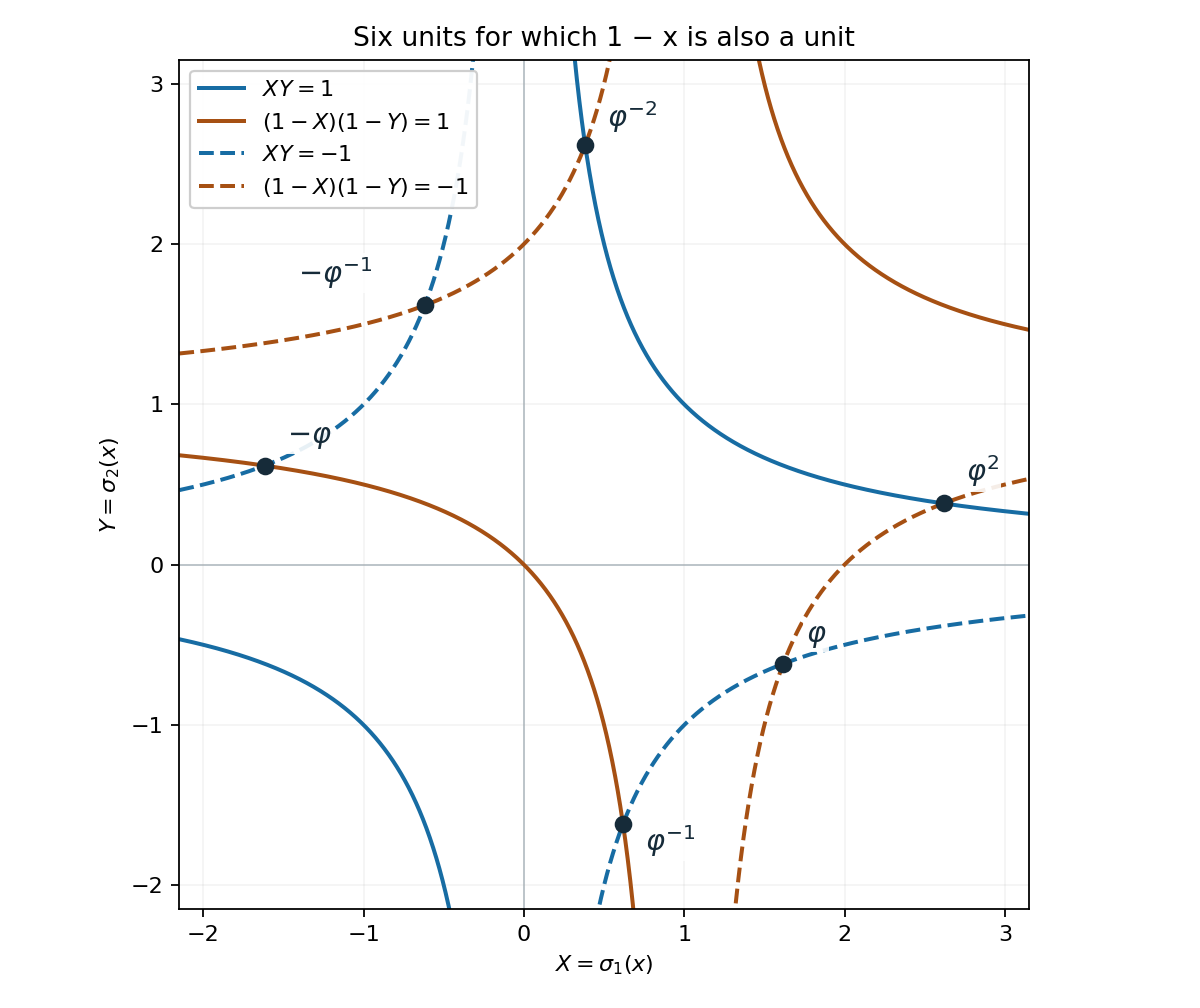
\includegraphics[keepaspectratio,alt={The six golden-ratio unit solutions as intersections of norm curves.}]{../figures/golden-ratio-norm-curves.png}}
\par\smallskip
\begin{flushleft}\small
\emph{Figure 12.1. In the real Minkowski coordinates
\((X,Y)=(\sigma_1x,\sigma_2x)\), the two norm conditions are \(XY=\pm1\)
and \((1-X)(1-Y)=\pm1\). Their six intersections are labelled by the
exact element \(x\); the corresponding \(y\) is \(1-x\). The plotted
curves and positions are numerical renderings of these exact equations.
Proposition 12.7 supplies the algebraic classification and proves that
every intersection displayed comes from a unit. The
\href{https://kokunoyumeto.github.io/open-math-courses-public/courses/TR-BAKER/figure_sources/golden-ratio-norm-curves.py}{reproducible figure
source} and
\href{https://kokunoyumeto.github.io/open-math-courses-public/courses/TR-BAKER/verification/golden-ratio-certificate.py}{integer-arithmetic
certificate} accompany the lesson.}
\end{flushleft}
\end{minipage}\par\medskip


\subsection{7. Baker's height formulation for a multiplicative
group}\label{bakers-height-formulation-for-a-multiplicative-group}

The exponent bound also has a formulation that does not depend on a
particular expression for a group element. We use the archimedean case
of the formulation in
\href{https://math.uchicago.edu/~fcale/papers/ICM.pdf}{Calegari,
Dimitrov and Tang, \emph{Arithmetic holonomy bounds and effective
Diophantine approximation}, Theorem 1.1 and the discussion on page 2}.
The proof here uses Corollary 12.3 and the programme's elementary
lattice and height results.

\textbf{Lemma 12.8 (height and group coordinates).} Let
\(\Gamma=\langle a_1,\ldots,a_t\rangle\subset K^\times\) be finitely
generated. One can effectively find elements \(g_1,\ldots,g_\rho\) whose
classes form a basis of \(\Gamma/(\Gamma\cap\mu_K)\), and positive
computable constants \(L_\Gamma,V_\Gamma\), such that \[
\gamma=\zeta\prod_{i=1}^{\rho}g_i^{b_i},\quad
\zeta\in\Gamma\cap\mu_K,\qquad
B:=\max_i|b_i|\le L_\Gamma h(\gamma),\qquad
h(\gamma)\le V_\Gamma B.
\tag{12.42}
\] For \(\rho=0\), all elements of \(\Gamma\) are torsion and have
height zero; the exponent assertions are omitted.

\textbf{Proof.} Enlarge a finite set \(S\) of places to contain all
infinite places and all prime ideals occurring in the principal
fractional ideals of the \(a_j\). Thus every element of \(\Gamma\) is an
\(S\)-unit. At infinite places use the logarithms from (12.19); at
finite \(\mathfrak p\in S\), use
\(-v_{\mathfrak p}(u)\log N\mathfrak p\). Write \(\lambda_S(u)\) for the
resulting real vector. The product formula and height definition give \[
\sum_{v\in S}\lambda_S(u)_v=0,\qquad
2d h(u)=\sum_{v\in S}|\lambda_S(u)_v|.
\tag{12.43}
\] The kernel is exactly the roots of unity: zero logarithms mean height
zero, and \emph{Heights of algebraic numbers}, Theorem 2.7, proves the
height-zero characterization.

The subgroup \(\lambda_S(\Gamma)\) is discrete. Indeed a bounded set of
logarithm vectors bounds height by (12.43), and Northcott leaves only
finitely many possible elements of \(K\), hence finitely many vectors.
The lattice structure lemma in \emph{Number fields}, \emph{Lattices,
Minkowski's theorem and the Minkowski embedding}, therefore identifies
this group with a lattice in its real span. Its rank \(\rho\) equals the
real dimension of that span.

We give an effective way to identify the basis; merely saying that a
basis exists would not settle the effective assertion. Form the real
matrix \(M\) whose columns are \(\lambda_S(a_j)\). Its integer kernel is
\[
R=\left\{c\in\mathbb Z^t:
                  \prod_j a_j^{c_j}\in\mu_K\right\}.
\tag{12.44}
\] It is saturated: if \(nc\in R\) for a nonzero integer \(n\), a power
of \(\prod_j a_j^{c_j}\) is a root of unity, so that element itself is a
root of unity.

Membership in \(R\) is decidable by exact arithmetic. Northcott's
explicit bound at height zero gives \[
\#\mu_K\le T:=d^2(2^{d+1}+1)^{d+1}.
\] The order of every root of unity is at most \(T\); hence
\(u\in\mu_K\) if and only if \(u^{T!}=1\). This supplies a finite exact
test for each candidate relation. There is no reliance on a numerical
test for a logarithm being zero.

Here is a terminating search for the rank and the whole kernel. For each
\(k=0,\ldots,t\), interleave the following two finite-certificate
searches: \(t-k\) rationally independent integer vectors in \(R\), and a
certified nonzero \(k\)-row, \(k\)-column minor of \(M\). The empty
minor is one. Enumerate relation vectors in growing integer boxes, using
the exact test just described. Approximate the entries of \(M\) with
certified rational intervals of successively smaller width; a nonzero
minor is eventually enclosed in an interval excluding zero. The
finite-place entries are integer multiples of logarithms of positive
integers. The infinite-place entries are logarithms of positive
algebraic moduli. These can be enclosed to arbitrary precision by
isolating the algebraic numbers and integrating \(1/t\) on a positive
interval; thus the interval tests are effective.

When both certificates occur for the same \(k\), the first gives
\(\operatorname{rank}M\le k\) and the second gives the reverse
inequality. For the actual rank \(\rho\), both certificates exist, by
the lattice structure just proved. The search therefore terminates. The
\(t-\rho\) found relations span the whole real kernel; intersecting
their rational span with \(\mathbb Z^t\) recovers \(R\), since \(R\) is
saturated. The integer Smith operations proved in \emph{Discriminants
and integral bases}, \emph{Integer subgroups and lattice indices},
compute this intersection and extend its basis to a basis of
\(\mathbb Z^t\). The remaining \(\rho\) vectors give the desired \(g_i\)
by taking the corresponding products of the \(a_j\).

The finite set \(S\) used in this construction is also effective: clear
denominators of the \(a_j\) in an integral basis and factor their
nonzero principal integral ideals. This can be done by a finite search
among additive subgroups of bounded index: ideal membership and
maximality are tests in the finite quotient, and the prime-ideal
factorization theorem then supplies the valuations. Thus no uncomputed
infinite support is hidden in the matrix \(M\).

Choose any nonzero \(\rho\)-row minor \(E\) of the logarithm matrix of
the \(g_i\). It is square and invertible. A certified interval
calculation gives an integer \(L_\Gamma\ge1\) larger than \(d\) times
every absolute row sum of \(E^{-1}\). Since each coordinate of
\(\lambda_S(\gamma)\) is at most \(dh(\gamma)\) in absolute value,
solving for \(b\) proves the first bound in (12.42). Choose a computable
\(V_\Gamma\ge1\) with \(V_\Gamma\ge\sum_i h(g_i)\). The height product
inequality proves the second bound. Both constants are computed from the
fixed group generators and the field. \(\square\)

\textbf{Theorem 12.9 (Baker's height bound, archimedean form).} Fix a
number field \(K\), a complex embedding \(\sigma\), a finitely generated
subgroup \(\Gamma\subset K^\times\), and \(\epsilon>0\). There is a
computable constant \(C_\Gamma>0\), depending only on these fixed data,
such that for every \(A\in K^\times\) and \(\gamma\in\Gamma\), \[
|\sigma(1-A\gamma)|\le e^{-\epsilon h(\gamma)}
\quad\Longrightarrow\quad
h(\gamma)\le C_\Gamma\max\{h(A),1\}.
\tag{12.45}
\] The case \(A\gamma=1\) is included.

\textbf{Proof.} If \(A\gamma=1\), then \(h(\gamma)=h(A)\). If \(\gamma\)
is torsion, its height is zero. These cases are settled by
\(C_\Gamma\ge1\).

Otherwise use Lemma 12.8 to write \(\gamma=\zeta\prod_i g_i^{b_i}\),
with \(B\ge1\). The first inequality in (12.42) gives \[
0<\left|\sigma(A\zeta)\prod_i(\sigma g_i)^{b_i}-1\right|
\le e^{-\epsilon h(\gamma)}
\le e^{-\epsilon B/L_\Gamma}
<e^{-\epsilon B/(2L_\Gamma)}.
\tag{12.46}
\] Apply Corollary 12.3 with \(\delta=\epsilon/(2L_\Gamma)\) and varying
factor \(\eta=\sigma(A\zeta)\). Its height is \(h(A)\). If \(C_*\) is
the explicit constant there, then \[
B<C_*\max\{h(A),1\},\qquad
h(\gamma)\le V_\Gamma B.
\] Taking \(C_\Gamma=1+V_\Gamma C_*\) proves (12.45). The constants
depend only on the fixed data, not on \(A\). \(\square\)

For the height-normalized archimedean absolute value
\(|u|_v=|\sigma u|^{n_v/d}\), replace \(\epsilon\) in the theorem by
\(d\epsilon/n_v\). This proves the same statement with
\(|1-A\gamma|_v\le e^{-\epsilon h(\gamma)}\). Thus the normalized and
ordinary complex formulations agree after an explicit change of
parameter. The nonarchimedean statement requires a separate argument; no
such case is asserted here.

\subsection{8. Fundamental units with regulator
bounds}\label{fundamental-units-with-regulator-bounds}

The degree-and-discriminant estimates already prove the unit equation.
We now give the more precise fundamental-system statement in terms of
the regulator, including its geometric ingredients. The free sources are
\href{https://arxiv.org/abs/math/0204158}{Henk, \emph{Successive Minima
and Lattice Points}, Section 3} and
\href{https://matwbn.icm.edu.pl/ksiazki/aa/aa74/aa7416.pdf}{Bugeaud and
Győry, \emph{Bounds for the solutions of unit equations}, Lemma 1}. Our
height \(h\) is logarithmic throughout.

\textbf{Lemma 12.10 (Minkowski's second upper bound).} Let
\(C\subset\mathbb R^n\) be compact, convex, symmetric about zero and
have nonempty interior. Let \(\Lambda\) be a full lattice and let
\(0<\lambda_1\le\cdots\le\lambda_n\) be the successive minima of \(C\):
\(\lambda_i\) is the least dilation containing \(i\) independent lattice
vectors. Then \[
\lambda_1\cdots\lambda_n\,\operatorname{vol}(C)
\le 2^n\det\Lambda.
\tag{12.47}
\]

\textbf{Proof.} A linear change of variables first makes
\(\Lambda=\mathbb Z^n\); it divides volume by \(\det\Lambda\) and leaves
the minima unchanged. The minima are attained because a bounded set has
finitely many lattice points. Choose independent \(v_i\in\lambda_i C\),
with the first \(i\) vectors spanning \(F_i\).

We can choose a lattice basis adapted to the flag
\(F_1\subset\cdots\subset F_n\). Indeed \(\mathbb Z^n\cap F_i\) is
saturated, and so is \((\mathbb Z^n\cap F_{i-1})\) inside it. Their
quotient is free of rank one. The integer basis-extension argument from
Lemma 12.4, or the proved Smith operations, therefore extends the bases
one step at a time. In these unimodular coordinates \(F_i\) is the
subspace on the first \(i\) coordinate axes. This change preserves
volume and the integer lattice; it need not be orthogonal.

Put \(C_i=(\lambda_i/2)C\), and, for a positive integer \(q\), let \[
Z_q=\{-q,\ldots,q\}^n,\qquad Z_q^{(i)}=Z_q\cap F_i.
\tag{12.48}
\] The translates \(z+\operatorname{int}C_1\), \(z\in\mathbb Z^n\), are
disjoint: an overlap would put a nonzero lattice difference in
\(\operatorname{int}(\lambda_1 C)\). Boundaries of convex bodies have
volume zero. Consequently \[
\operatorname{vol}(Z_q+C_1)
=(2q+1)^n(\lambda_1/2)^n\operatorname{vol}(C).
\tag{12.49}
\] The boundedness of \(C_n\) also gives a constant \(c\), independent
of \(q\), such that \(\operatorname{vol}(Z_q+C_n)\le(2q+c)^n\).

We show that, for \(i<n\), \[
\operatorname{vol}(Z_q+C_{i+1})
\ge(\lambda_{i+1}/\lambda_i)^{n-i}
       \operatorname{vol}(Z_q+C_i).
\tag{12.50}
\] Equal consecutive minima give equality, so assume
\(t=\lambda_{i+1}/\lambda_i>1\). Two integer translates of
\(\operatorname{int}C_{i+1}\) whose last \(n-i\) coordinates differ
cannot intersect. Otherwise their nonzero difference lies outside
\(F_i\) and in \(\operatorname{int}(\lambda_{i+1}C)\); together with
\(v_1,\ldots,v_i\), which also lie in that interior because
\(\lambda_i<\lambda_{i+1}\), it gives \(i+1\) independent vectors at a
dilation smaller than \(\lambda_{i+1}\). This is impossible.

Partition \(Z_q\) according to its last \(n-i\) coordinates. The
corresponding clusters of translates have disjoint interiors. For
\(j=i,i+1\), therefore, \[
\operatorname{vol}(Z_q+C_j)
=(2q+1)^{n-i}\operatorname{vol}(Z_q^{(i)}+C_j).
\tag{12.51}
\] Write a vector as \((x,y)\in F_i\oplus F_i^\perp\). Define
\(A_t(x,y)=(tx,y)\) and \(B_t(x,y)=(x,ty)\). Then \(C_{i+1}=B_tA_tC_i\),
and \(B_t\) fixes \(Z_q^{(i)}\). It remains to prove \[
\operatorname{vol}(Z_q^{(i)}+A_tC_i)
\ge\operatorname{vol}(Z_q^{(i)}+C_i).
\tag{12.52}
\]

For fixed \(y\), let \(D_y=\{x:(x,y)\in C_i\}\). If it is nonempty,
choose any \(b\in D_y\). Convexity gives the explicit containment \[
D_y+(t-1)b\subseteq tD_y:
\quad
\frac{x+(t-1)b}{t}=\frac{x}{t}+
                    \left(1-\frac1t\right)b\in D_y
\quad(x\in D_y).
\tag{12.53}
\] Adding the finite set \(Z_q^{(i)}\) preserves containment. Thus the
\(i\)-dimensional volume of the slice of \(Z_q^{(i)}+A_tC_i\) is at
least that of the corresponding slice of \(Z_q^{(i)}+C_i\). Empty slices
cause no problem. Integration of the slice volumes proves (12.52).

Here only the elementary slice formula for a finite union of convex
bodies is needed. To verify it directly, enclose such a bounded set
between the unions of grid boxes lying inside it and meeting it. The
difference has volume tending to zero with the mesh: for a convex body
containing a ball of radius \(\rho\) about an interior point, the
boundary layer of thickness \(a\) is contained between its
\((1-a/\rho)\)- and \((1+a/\rho)\)-dilates about that point. The
difference of their volumes tends to zero. A finite union inherits this
property. For a finite union of grid boxes, the slice identity is just
the product formula for box volumes and finite addition. The lower and
upper box sums squeeze both the volume and the integral of the slice
volumes to the same number. The same argument proves that the boundaries
used in (12.49) and (12.51) have volume zero. This establishes the slice
step without assuming a general product measure theorem.

Now \(B_t\) multiplies volume by \(t^{n-i}\); combining (12.51) and
(12.52) proves (12.50). Multiplying (12.50) for \(i=1,\ldots,n-1\) and
using (12.49) gives \[
(2q+c)^n\ge
\frac{\lambda_1\cdots\lambda_n}{2^n}
       \operatorname{vol}(C)(2q+1)^n.
\tag{12.54}
\] The powers telescope, including when minima repeat. Divide by
\((2q+1)^n\) and let \(q\) tend to infinity. This proves (12.47) for
\(\mathbb Z^n\); reversing the first linear change proves it for
\(\Lambda\). The case \(n=1\) uses (12.49) directly. \(\square\)

\textbf{Lemma 12.11 (a basis adapted to the minima).} Let \(F\) be a
norm on \(\mathbb R^r\), let \(\Lambda\) be a full lattice, and let
\(\lambda_i\) be its successive minima for \(F\). There is a lattice
basis \(b_1,\ldots,b_r\) such that \[
F(b_i)\le\max\{1,i/2\}\lambda_i.
\tag{12.55}
\]

\textbf{Proof.} Choose independent \(v_i\) with \(F(v_i)=\lambda_i\),
and put \(\Lambda_i=\Lambda\cap\operatorname{span}_{\mathbb R}
(v_1,\ldots,v_i)\). Each quotient \(\Lambda_i/\Lambda_{i-1}\) is
infinite cyclic, by saturation and the integer subgroup theorem. Choose
a generator represented by \(w\). After changing its sign, the image of
\(v_i\) is \(k\) times that generator, for some integer \(k\ge1\).

If \(k=1\), take \(b_i=v_i\). If \(k\ge2\), express \[
w=\frac1k v_i+\sum_{j<i}a_jv_j
\] with real \(a_j\), and subtract integer multiples of the \(v_j\) to
make all \(|a_j|\le1/2\). This leaves a generator of the quotient. Call
the resulting vector \(b_i\). Then \[
F(b_i)\le\frac{\lambda_i}{k}
                +\frac12\sum_{j<i}\lambda_j
          \le\frac i2\lambda_i.
\] Choose these quotient generators successively. Since the preceding
basis spans \(\Lambda_{i-1}\), adjoining \(b_i\) gives a basis of
\(\Lambda_i\). At \(i=r\) it is a basis of \(\Lambda\). When \(i=1\),
shortestness forces \(k=1\); the construction also covers repeated
minima. \(\square\)

\textbf{Theorem 12.12 (quantitative fundamental systems).} Let \(S\) be
a finite set of places of \(K\) containing all infinite places, let
\(s=|S|\ge2\), and set \(r=s-1\), \(d=[K:\mathbb Q]\). Use the unscaled
logarithms in (12.43). Let \(R_S\) be the absolute determinant obtained
by deleting one row from the logarithm matrix of a fundamental system of
\(S\)-units. Suppose \(\delta>0\) is a known constant such that \[
h(u)\ge\delta/d
\quad\text{for every non-torsion }u\in O_{K,S}^{\times}.
\tag{12.56}
\] Put \[
c_4=\frac{(r!)^2}{2^{r-1}d^r},\qquad
c_5=c_4(d/\delta)^{r-1},\qquad
c_6=\frac{c_4d^r}{\delta}.
\tag{12.57}
\] For any chosen omitted place there is a fundamental system
\(\varepsilon_1,\ldots,\varepsilon_r\) such that \[
\prod_{i=1}^r h(\varepsilon_i)\le c_4R_S,\qquad
h(\varepsilon_i)\le c_5R_S,
\tag{12.58}
\] and every entry of the inverse of its deleted-row logarithm matrix
has absolute value at most \(c_6\). The choice may depend on the omitted
place.

An admissible explicit height-gap parameter, depending only on \(d\), is
\[
P_d=d^2(2\cdot3^d+1)^d,\qquad \delta=\frac1{2P_d}.
\tag{12.59}
\]

\textbf{Proof.} The programme's \(S\)-unit theorem (\emph{Number
fields}, Theorem 9.4) gives \(O_{K,S}^\times/\mu_K\) rank \(r\).
Equation (12.43), Northcott and the height-zero theorem make its
logarithm image a discrete rank-\(r\) subgroup of the sum-zero
hyperplane. Thus it is a full lattice there. Deleting the chosen
coordinate identifies it with a lattice \(\Lambda\subset\mathbb R^r\).
Changing the fundamental system changes the determinant by a sign;
changing the omitted row also changes it only by a sign, because all
rows sum to zero. This proves the asserted meaning of \(R_S\) and gives
\(\det\Lambda=R_S\).

Use the norm \(F(z)=|z_1|+\cdots+|z_r|\). Its unit ball has volume
\(2^r/r!\): each orthant contributes the simplex
\(\{z_j\ge0,\sum z_j\le1\}\), whose volume is \(1/r!\) by repeated
integration, and the orthants have disjoint interiors. Lemma 12.10 gives
\(\prod_i\lambda_i\le r!R_S\). Lemma 12.11 then supplies a basis with \[
\prod_iF(b_i)\le
\left(\prod_{i=1}^r\max\{1,i/2\}\right)\prod_i\lambda_i
\le\frac{(r!)^2}{2^{r-1}}R_S=c_4d^rR_S.
\tag{12.60}
\] Lift it to \(S\)-units \(\varepsilon_i\). Since the missing
coordinate is minus the sum of the retained ones, (12.43) gives \[
\frac{F(b_i)}{2d}\le h(\varepsilon_i)
                       \le\frac{F(b_i)}d.
\tag{12.61}
\] Multiplying the upper inequalities proves the first assertion in
(12.58). Divide that product bound by the lower bounds
\((\delta/d)^{r-1}\) for the other factors to obtain the second.

For the inverse estimate, put the \(b_i\) in columns of \(E\). Delete
column \(i\) and any row. The determinant expansion, followed by the
triangle inequality, is bounded by \(\prod_{j\ne i}F(b_j)\): expanding
this product sums all choices of row indices, including all the distinct
choices in the determinant. Equation (12.60) bounds the cofactor by
\(c_4d^rR_S/F(b_i)\). Since \(F(b_i)\ge d h(\varepsilon_i)\ge\delta\),
division by \(|\det E|=R_S\) gives the bound \(c_6\).

It remains to justify (12.59). The bounded-powers argument in Lemma 12.5
applies to every nonzero algebraic integer of degree at most \(d\), not
just to units: if its height were at most \(\log2/(dP_d)\), the
\(P_d+1\) powers would belong to the same finite set of at most \(P_d\)
algebraic integers with conjugates bounded by two. A repeated power
would make it torsion. For a nonintegral algebraic number, the positive
leading coefficient of its primitive minimal polynomial is at least two.
The proved Mahler-measure formula in \emph{Heights of algebraic
numbers}, Theorem 2.4, then gives \(h(u)\ge\log2/\deg(u)\ge\log2/d\).
Since \(\log2>1/2\), both cases imply (12.56) with (12.59). \(\square\)

For ordinary units \(S=S_\infty\), this is the precise regulator-based
fundamental-system estimate. Lemma 12.5 gives a separate uniform
degree-and-discriminant bound for the same regulator: the determinant
expansion for its basis, whose coordinates have absolute value at most
\(V\), gives \[
R_K\le r!V^r.
\tag{12.62}
\] Consequently the system in Theorem 12.12 also has heights bounded
explicitly in terms of \(d,\Delta\), by (12.57)--(12.59) and (12.62).
Its exponent coordinates satisfy \(\max_i|b_i|\le rd\,c_6h(u)\), by
solving the logarithm system. These statements specify both the
bounded-unit input and the height-to-exponent conversion used in
applications.

If \(s=1\), the \(S\)-unit rank is zero, every \(S\)-unit is torsion,
and there is no logarithm matrix to invert. That case is covered
separately, rather than by formulas containing \(r-1=-1\).

\subsection{9. Finiteness, height bounds and stopping a
search}\label{finiteness-height-bounds-and-stopping-a-search}

The distinction between a finite solution set and a computably bounded
one is visible in the earlier programme proofs.
\href{https://kokunoyumeto.github.io/open-math-courses-public/courses/TR-TRANS/TR-TRANS-12.html\#theorem-12-1-roth-s-theorem}{Roth's
theorem, \emph{Roth's theorem and its consequences}, Theorem 12.1}
states that, for a real irrational algebraic number \(\theta\) and
\(\epsilon>0\), only finitely many reduced \(p/q\), \(q>0\), satisfy \[
|\theta-p/q|<q^{-2-\epsilon}.
\tag{12.63}
\] Its proof assumes infinitely many exceptions and selects denominators
successively far apart. The contradiction rules out that infinite
supply. It does not compute a largest exceptional denominator. This
precise limitation is explained in
\href{https://kokunoyumeto.github.io/open-math-courses-public/courses/TR-TRANS/TR-TRANS-12.html\#4-why-the-proof-gives-finiteness-without-a-denominator-bound}{Section
4 of that lesson}. It does not mean that every individual approximation
problem is ineffective; a particular problem can admit additional
arguments.

For unit equations the comparison is the following programme theorem.
Let \(K\) be a number field, let \(S\) be finite and contain the
infinite places, and fix \(a_1,\ldots,a_n\in K^\times\). There are
finitely many solutions \[
a_1u_1+\cdots+a_nu_n=1,\qquad u_i\in O_{K,S}^\times,
\tag{12.64}
\] for which no nonempty subsum on the left vanishes. Equivalently, a
homogeneous equation in \(m\) nonzero terms has finitely many projective
solution tuples if no nonempty proper subsum vanishes. The complete
proof is
\href{https://kokunoyumeto.github.io/open-math-courses-public/courses/TR-TRANS/TR-TRANS-12.html\#corollary-12-17-nondegenerate-s--unit-equations}{\emph{Roth's
theorem and its consequences}, Corollary 12.17}, using the
\href{https://kokunoyumeto.github.io/open-math-courses-public/courses/TR-TRANS/TR-TRANS-12.html\#theorem-12-13-the-projective-subspace-theorem}{projective
Subspace theorem proved there as Theorem 12.13}.

The role of the Subspace theorem in that proof is precise. At each
place, replace a coordinate of largest absolute value by the sum of the
coordinates. The product formula makes the resulting product of linear
forms small enough for the Subspace theorem. Its finitely many proper
subspaces give homogeneous relations with fewer terms. Minimal vanishing
subsums and induction then give finiteness. The proof supplies no
explicit height cutoff for all solutions.

For two terms, nondegeneracy is automatic: each individual term is
nonzero, and their sum is one. Thus the qualitative theorem includes our
ordinary unit equation. Theorem 12.6 supplies the further information
needed for an exhaustive search: the computed bound
\(C_{\rm unit}(d,\Delta)\max\{h(\alpha),h(\beta),1\}\). The coefficient
dependence is linear, and the proof displays every constant before any
solution is selected.

For three terms, the restriction is indispensable. In the golden-ratio
field the tuples \((\varphi^j,-\varphi^j,1)\), \(j\in\mathbb Z\), are
distinct unit solutions of \(u_1+u_2+u_3=1\), but the first two terms
cancel. There is no conflict with the theorem.

Theorem 12.6 concerns ordinary units. The regulator statement in Theorem
12.12 also covers \(S\)-units, but that alone does not extend the proof
of Theorem 12.6: for an \(S\)-unit, a small place can be finite, where
the complex two-logarithm estimate does not apply. The later lesson on
\(S\)-unit and Thue--Mahler equations combines the archimedean and
nonarchimedean estimates.

\subsection{10. Exercises}\label{exercises}

\begin{enumerate}
\def\labelenumi{\arabic{enumi}.}
\item
  \textbf{Easy --- two rank-zero rings.} Prove that \(x+y=1\) has no
  solution in units of \(\mathbb Z\), and none in units of
  \(\mathbb Z[i]\). Determine the unit groups as part of the proof.
\item
  \textbf{Medium --- simultaneous approximation with rounding.} Prove
  Lemma 12.1 from the compact form of Minkowski's convex body theorem.
  Include \(Q=1\), zero and negative \(b_i\), and the denominator
  \(2r-1\). For \(b=(1001,-997,2503)\), \(N=64\), \(Q=27\), verify the
  displayed choice \(p_0=2\), \(p=(31,-31,78)\), \(r=32\).
\item
  \textbf{Medium --- from exponents to Baker's height formulation.} Let
  \(\Gamma\subset K^\times\) be finitely generated, and fix a complex
  embedding and \(\epsilon>0\). Starting from Corollary 12.3 and Lemma
  12.8, prove Theorem 12.9. Treat the non-strict inequality, torsion and
  exact equality \(A\gamma=1\), and show how normalized archimedean
  absolute values change the parameter.
\item
  \textbf{Hard --- every golden-ratio solution.} Give explicit integer
  constants bounding the exponents in \(x+y=1\),
  \(x,y\in\mathbb Z[\varphi]^\times\), using Theorem 12.6. Reduce the
  exponent box by norm and trace, perform an exact finite search and
  prove that the six ordered pairs in (12.37) are complete.
\item
  \textbf{Medium --- a rank-one regulator check.} Let
  \(K=\mathbb Q(\sqrt5)\), \(S=S_\infty\), and omit either real place.
  Compute \(R_K\), the height of the fundamental unit and the inverse
  logarithm matrix. Verify Theorem 12.12 with the admissible gap
  \(\delta=\log\varphi\).
\item
  \textbf{Medium --- why a generating system is not enough.} For
  \(r\ge3\), let \[
  \Lambda=\mathbb Z^r+\mathbb Z(1/2,\ldots,1/2).
  \] With the \(\ell^1\)-norm, find its successive minima and show that
  the standard unit vectors need not be a lattice basis. Construct a
  basis satisfying Lemma 12.11 and compute its determinant.
\item
  \textbf{Medium --- finiteness and a stopping rule.} Explain why a
  bound on the number of exceptional rationals in Roth's theorem would
  not by itself tell an enumeration where to stop. Explain why Theorem
  12.6 does provide a stopping rule, and give the degenerate infinite
  family showing why (12.64) needs its subsum condition.
\end{enumerate}

\subsection{11. Solutions}\label{solutions}

\textbf{1.} An integer unit divides one, so it is \(1\) or \(-1\). Their
pairwise sums are \(2,0,-2\). In \(\mathbb Z[i]\), the multiplicative
norm \(N(a+bi)=a^2+b^2\) is a positive integer on nonzero elements. A
unit has norm one, and conversely a norm-one element has its conjugate
as inverse. Thus the units are \(1,-1,i,-i\). If \(x=1\), then
\(1-x=0\); if \(x=-1\), then \(1-x=2\); if \(x=\pm i\), then
\(N(1-x)=2\). None of these values is a unit.

\textbf{2.} For \(Q>1\), use the body (12.2). The shear in the proof of
Lemma 12.1 gives volume \(2^{n+1}\), so Minkowski gives a nonzero
integer point. Its first coordinate cannot vanish, because
\(Q^{-1/n}<1\); change signs to arrange \(1\le p_0\le Q\). Put
\(t=N/p_0\) and round it to a nearest integer \(r\). Then
\(\lfloor N/Q\rfloor\le r\le N\), \(r\ge1\), and \[
|b_i-rp_i|
\le r|b_i/t-p_i|+|b_i||t-r|/t
\le rQ^{-1/n}+\frac{|b_i|}{2r-1}.
\] Only absolute values of the \(b_i\) were used, so signs and zero
coordinates are covered. For \(Q=1\), take \(r=N\) and round \(b_i/N\);
the error is at most \(N/2\), which is below the first term of the
required bound. In the example the three errors \(p_0b_i/N-p_i\) are
\(9/32,-5/32,7/32\), all of modulus below \(1/3\). Multiplication by
\(r=32\) gives the remainder vector \((9,-5,7)\); the three final bounds
also follow directly from \(r/3+|b_i|/63\).

\textbf{3.} If \(A\gamma=1\), then \(h(\gamma)=h(A)\). Torsion has
height zero. Otherwise write \(\gamma=\zeta\prod_i g_i^{b_i}\) with the
basis of Lemma 12.8. Its exponent maximum \(B\) is positive, and
\(B\le L_\Gamma h(\gamma)\), \(h(\gamma)\le V_\Gamma B\). The assumed
error satisfies \[
0<\left|\sigma(A\zeta)\prod_i(\sigma g_i)^{b_i}-1\right|
\le e^{-\epsilon B/L_\Gamma}
<e^{-\epsilon B/(2L_\Gamma)}.
\] Corollary 12.3 with \(\delta=\epsilon/(2L_\Gamma)\) therefore gives
\(B<C_*\max\{h(A),1\}\), since roots of unity and embeddings preserve
height. Hence \(C_\Gamma=1+V_\Gamma C_*\) works in all cases. All data
entering \(C_*\) are fixed group generators and the fixed parameter. If
\(|u|_v=|\sigma u|^{n_v/d}\), raising the assumed inequality to
\(d/n_v\) replaces \(\epsilon\) by \(d\epsilon/n_v\). This proves
exactly the normalized archimedean statement.

\textbf{4.} The constants can be given without decimal approximations.
Specializing (12.21) and (12.31), take \[
\begin{gathered}
V=256\cdot10^{11},\qquad P=1444,\qquad L=4V^2(8P)^2,\\
S_0=4V+15,\qquad C_0=259200S_0(2S_0+1),\\
q_0=(4800C_0L)^2,\qquad
G=2V(8L+28q_0^5)+11.
\end{gathered}
\tag{12.65}
\] These are positive integers and \(G=C_{\rm unit}(2,5)\). As
\(h(\pm\varphi^j)=|j|\log\varphi/2\) and \(\log\varphi>2/5\), Theorem
12.6 first gives \(|j|,|k|<5G\). This is an effective finite box before
the following reduction.

Put \(s=N(x)\), \(t=N(1-x)\), so \(s,t=\pm1\). The trace is \(1+s-t\),
and both conjugates of \(x\) are roots of (12.39). Their absolute values
are less than four; their product has modulus one, so both have modulus
greater than \(1/4\). The same holds for \(y\). Since \(\varphi^3>4\),
only \(-2\le j,k\le2\) remain. Enumerate the ten signed powers in that
range by the integer-pair multiplication (12.41), and test their one
hundred ordered sums against \((1,0)\). The six successes are exactly
the rows of the table in Section 6. The four norm polynomials there give
an independent hand check: the \((1,1)\) case has no real roots, and
each of the other three cases has the two listed roots. Thus the
reduction excludes every exponent outside the finite box, and the exact
enumeration settles every candidate inside it.

\textbf{5.} The logarithm vector of \(\varphi\) is
\((\log\varphi,-\log\varphi)\); hence \(R_K=\log\varphi\) and
\(h(\varphi)=R_K/2\). Every non-torsion unit is \(\pm\varphi^j\),
\(j\ne0\), so its height is at least \((\log\varphi)/2=\delta/d\). Here
\(r=1\), \(d=2\), and \[
c_4=c_5=\frac12,\qquad c_6=\frac1{\log\varphi}.
\] The product and individual height bounds are equalities. The
one-by-one deleted-row matrix is \((\log\varphi)\) or
\((-\log\varphi)\); its inverse has absolute entry \(c_6\). This checks
the normalization and the rank-one endpoint.

\textbf{6.} Every vector lies either in \(\mathbb Z^r\) or in the coset
with every coordinate half-integral. A nonzero integer vector has
\(\ell^1\)-norm at least one. A vector in the other coset has norm at
least \(r/2\ge3/2\). Since the \(r\) standard unit vectors have norm
one, all successive minima are one. They generate the index-two
sublattice \(\mathbb Z^r\), not \(\Lambda\). A full basis is \[
e_1,\ldots,e_{r-1},\quad w=(1/2,\ldots,1/2),
\] because \(e_r=2w-\sum_{i<r}e_i\). Its determinant is \(1/2\), its
first \(r-1\) vectors have norm one, and its last has norm \(r/2\).
These satisfy (12.55), including equality for the last vector. Thus
replacing independent short vectors by a genuine lattice basis is a
substantive step.

\textbf{7.} A cardinality bound limits how many exceptions occur, but
the last one could lie after an arbitrarily long gap. Finding fewer than
the bound does not certify that none remain. In Theorem 12.6, the
explicitly bounded heights give a finite list of possible minimal
polynomials by Northcott's coefficient argument, or a finite exponent
box once a fundamental system is given. Checking that whole list is a
stopping rule, including when there are no solutions. The family
\((\varphi^j,-\varphi^j,1)\) consists of infinitely many distinct unit
solutions of the three-term equation; its two-term vanishing subsum is
exactly what (12.64) excludes.

\subsection{References}\label{references}

\begin{itemize}
\tightlist
\item
  Yuri Bilu and Yann Bugeaud, \emph{Démonstration du théorème de
  Baker--Feldman via les formes linéaires en deux logarithmes}, Journal
  de Théorie des Nombres de Bordeaux 12 (2000), 13--23, Section 2.
  \href{https://numdam.org/item/JTNB_2000__12_1_13_0/}{Free Numdam
  edition}.
\item
  Yann Bugeaud and Kálmán Győry, \emph{Bounds for the solutions of unit
  equations}, Acta Arithmetica 74 (1996), 67--80, Lemma 1 and the
  unit-equation argument.
  \href{https://matwbn.icm.edu.pl/ksiazki/aa/aa74/aa7416.pdf}{Free
  journal PDF}.
\item
  Martin Henk, \emph{Successive Minima and Lattice Points},
  arXiv:math/0204158v1 (2002), Section 3.
  \href{https://arxiv.org/abs/math/0204158}{Free preprint}.
\item
  Frank Calegari, Vesselin Dimitrov and Yunqing Tang, \emph{Arithmetic
  holonomy bounds and effective Diophantine approximation} (2026),
  Theorem 1.1 and its archimedean formulation.
  \href{https://math.uchicago.edu/~fcale/papers/ICM.pdf}{Free
  author-hosted text}.
\end{itemize}

\end{document}
